%% %%%%%%%%%%%%%%%%%%%%%%%%%%%%%%%%%%%%%%%%% %%
%% Elementos Pós Textuais
%% ----------------------
%% 
%% Segundo o manual do IFPI, eles devem ser os seguintes (nessa ordem):
%% 1. Referências (obrigatório)
%% 2. Glossário (opcional)
%% 3. Apêndice (opcional)
%% 4. Anexos (opcional)
%% 5. Índices (opcional)
%% %%%%%%%%%%%%%%%%%%%%%%%%%%%%%%%%%%%%%%%%% %%

%% Indica ao LaTeX que a partir deste ponto ficarão os elementos pós-textuais
\postextual

%% 01: Referências bibliográficas
%% Referências bibliográficas

% \bibliography{bibliografia}
\printbibliography

%% 02: Glossário
%% Glossário
%\glossary

%% 03: Apêndices
%% Apêndices

%\begin{apendicesenv}
%
%%% Imprime uma página indicando o início dos apêndices (opcional, comente para retirar)
%\partapendices
%
%%% Cada Capítulo será um apêndice
%\chapter{Este será o apêndice A}
%Lorem ipsum dolor sit amet, consectetur adipiscing elit. Praesent congue, turpis quis rutrum fringilla, lacus lorem faucibus diam, sit amet viverra urna quam sed metus. Pellentesque quis eros ex. Nullam vel ante rutrum eros placerat egestas. Morbi volutpat sapien elementum tincidunt fringilla. Class aptent taciti sociosqu ad litora torquent per conubia nostra, per inceptos himenaeos. Sed rutrum vestibulum bibendum. Sed tincidunt, magna sit amet tempor tincidunt, turpis neque blandit eros, a tincidunt felis mauris vitae est. Aliquam sit amet placerat risus. Nunc eget est pulvinar est tristique convallis sit amet vel risus. Maecenas turpis nisl, blandit ac porttitor non, ultrices id est. Cras eleifend nulla ut condimentum ullamcorper. Quisque at gravida massa, fringilla varius sapien. Nulla ullamcorper mauris vel ipsum elementum, vel tincidunt ante pretium. Ut iaculis nunc ex, vitae elementum ante efficitur non. Pellentesque venenatis tristique odio, nec volutpat dui dapibus sit amet. Maecenas eu velit at arcu hendrerit sagittis vel a odio.
%
%Nulla gravida metus at gravida ultricies. Nulla auctor id mi id suscipit. Proin vestibulum metus non eros feugiat, ac blandit diam vestibulum. Sed in arcu eget mauris rhoncus semper. Integer dignissim dui quis massa vestibulum, luctus ultrices metus mollis. Sed aliquam leo hendrerit lacus ultricies efficitur. Praesent quis quam sed lorem tincidunt fringilla non interdum odio. Phasellus vel enim mattis, tempor arcu ut, pulvinar est. Sed ut tempus est. Fusce erat nisi, scelerisque quis tellus sit amet, lacinia sagittis libero. Sed ultrices odio ipsum, ut vestibulum nulla auctor in.
%
%
%
%
%
%\chapter{Este será o apêndice B}
%Lorem ipsum dolor sit amet, consectetur adipiscing elit. Integer malesuada elit vel lacus fringilla, in luctus orci finibus. Praesent eget augue et enim luctus cursus ut ac nisl. In lobortis tellus non mauris euismod, tempus hendrerit nisi euismod. Integer id magna sapien. Nunc urna magna, consequat sed vehicula quis, convallis non justo. Aliquam risus dolor, viverra quis dignissim eget, convallis id sapien. Ut id turpis suscipit, mollis quam sed, lacinia lacus. Donec ac nulla dui.
%
%
%\end{apendicesenv}

%% 04: Anexos
%% Anexos
\begin{anexosenv}

%% Imprime uma página indicando o início dos anexos (opcional, comente para retirar)
%\partanexos

% Exemplo de inclusão
% \input{pos-textual/anexo} 
\chapter{TRECHO DA CARTA DE PERO VAZ DE CAMINHA} \label{anexo:a}
\vspace{-2cm}
\begin{figure}[H]
	\caption*{}
	\begin{center}
	    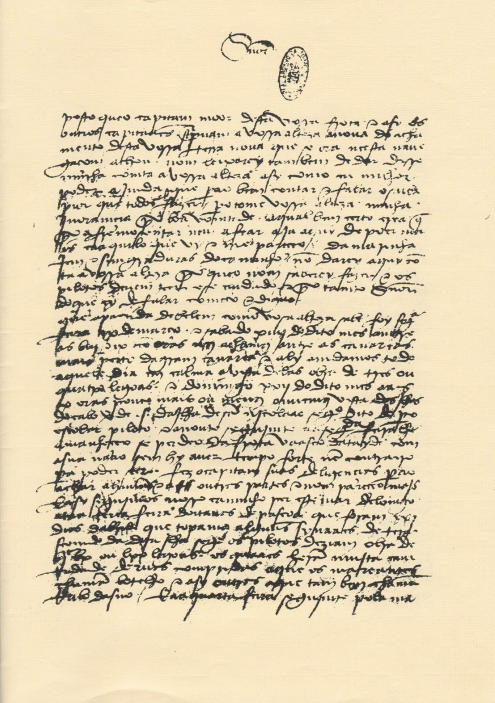
\includegraphics[scale=1.0]{imagens/carta_pero_vaz.png}
	\end{center}
	
\end{figure}


\end{anexosenv}

%% 05: Índices
%% Índices
%\phantompart \printindex

%% Capa do CD (opcional)
%%% Isso aqui cria a capa do CD, no final do documento :)
\newpage
\thispagestyle{empty}
\begin{center}
\covers[{\vspace{1.5cm} \Large \MakeUppercase{Curso de \imprimirnomedocurso} \\ \vspace{1cm} \textbf{\imprimirautor} \\ \vspace{0.5cm} {TÍTULO: \imprimirtitulo}}]{
	{\vspace{1.5cm} 
\includegraphics[scale=0.25]{imagens/IFPI.png} \\ \vspace{1cm} \MakeUppercase{Curso de \imprimirnomedocurso} \\ \vspace{1cm} {\textbf{\imprimirautor}} \\ \vspace{0.3cm} {TÍTULO: \imprimirtitulo} \\ \vspace{1.5cm} \MakeUppercase{\imprimirlocal} \par \imprimirdata}
}{
	\MakeUppercase{\tiny \imprimirtitulo}
}
\end{center}